%%%%%%%%%%%%%%%%%%%%%%%%%%%%%%%%%%%

%%% Background image
\ifthenelse{\equal{\detokenize{print-cover}}{\jobname}}{
  \backgroundsetup{
    scale=1,
    angle=0,
    opacity=1,
    position=current page.north west,
    nodeanchor=north west,
    % For some reason, current page.north east is 0.25in too high. This
    % is probably a bug related to the presence of bleed.
    contents={%
      \raisebox{-0.25in}[\height][0in]{%
        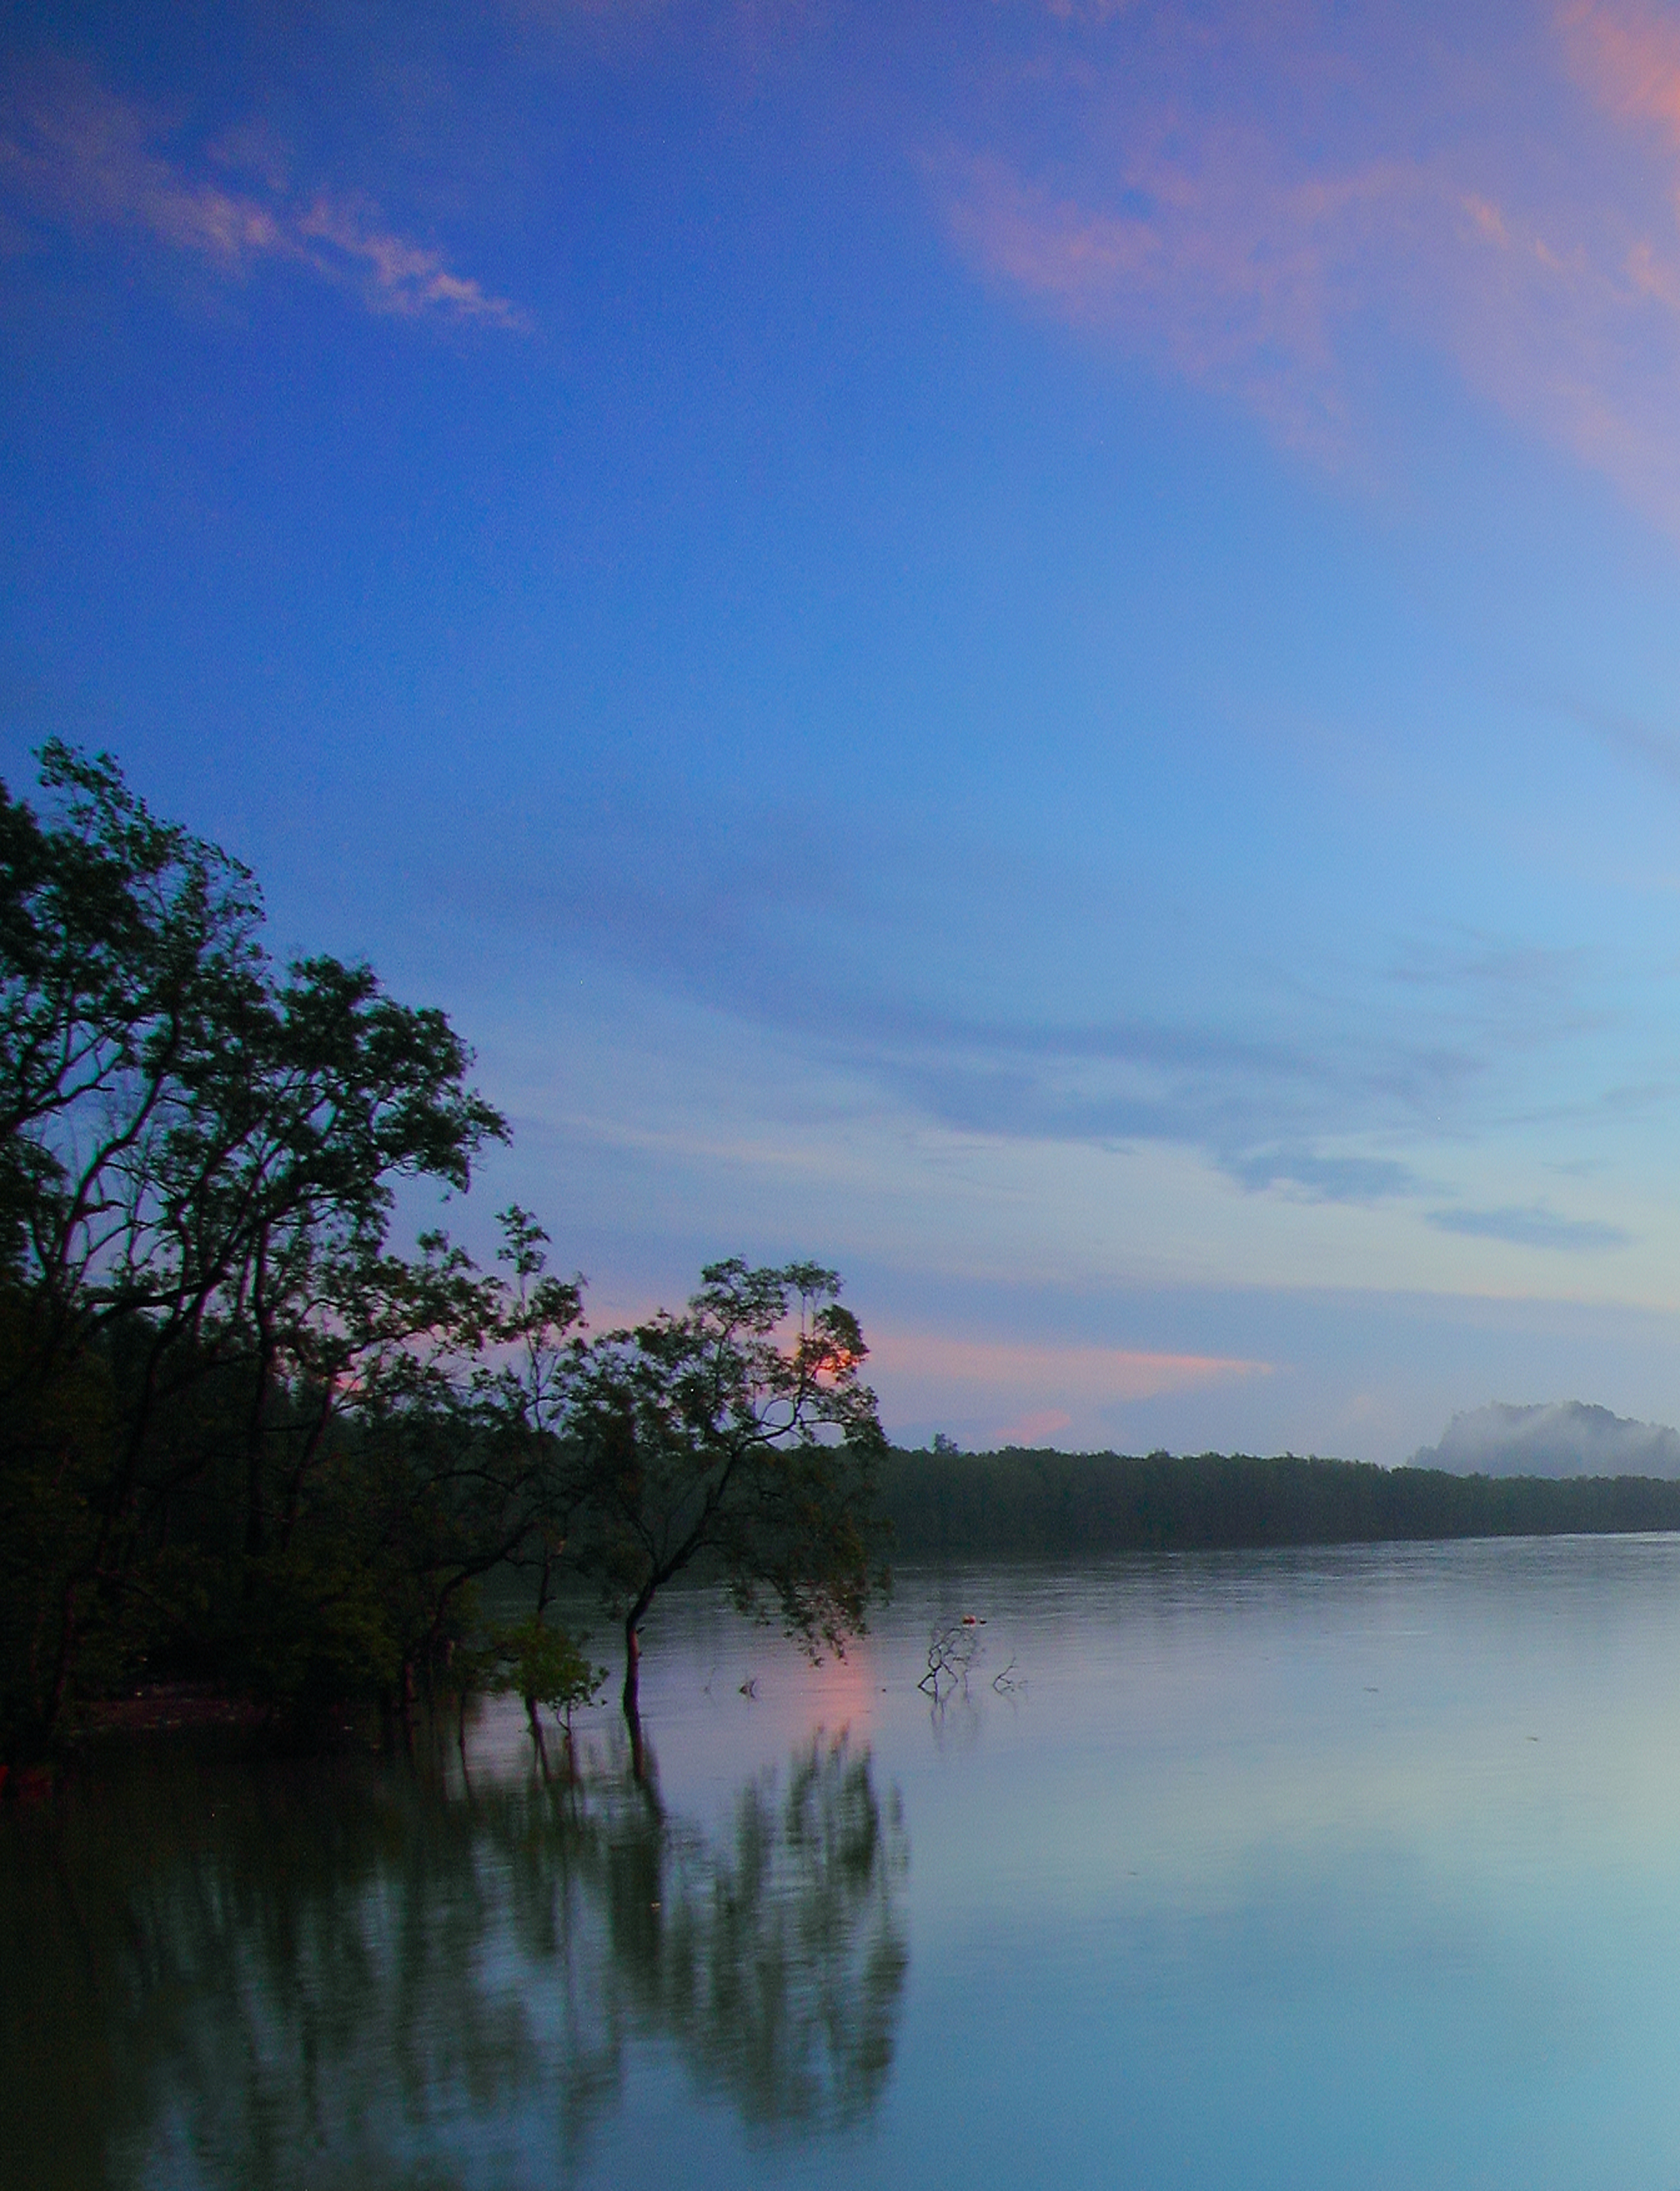
\includegraphics[height=\paperheight,width=8.5in+\bleed]{figures/titlepage-image-print2}%
        
\includegraphics[height=\paperheight,width=\spinewidth]{figures/titlepage-image-spine}%
        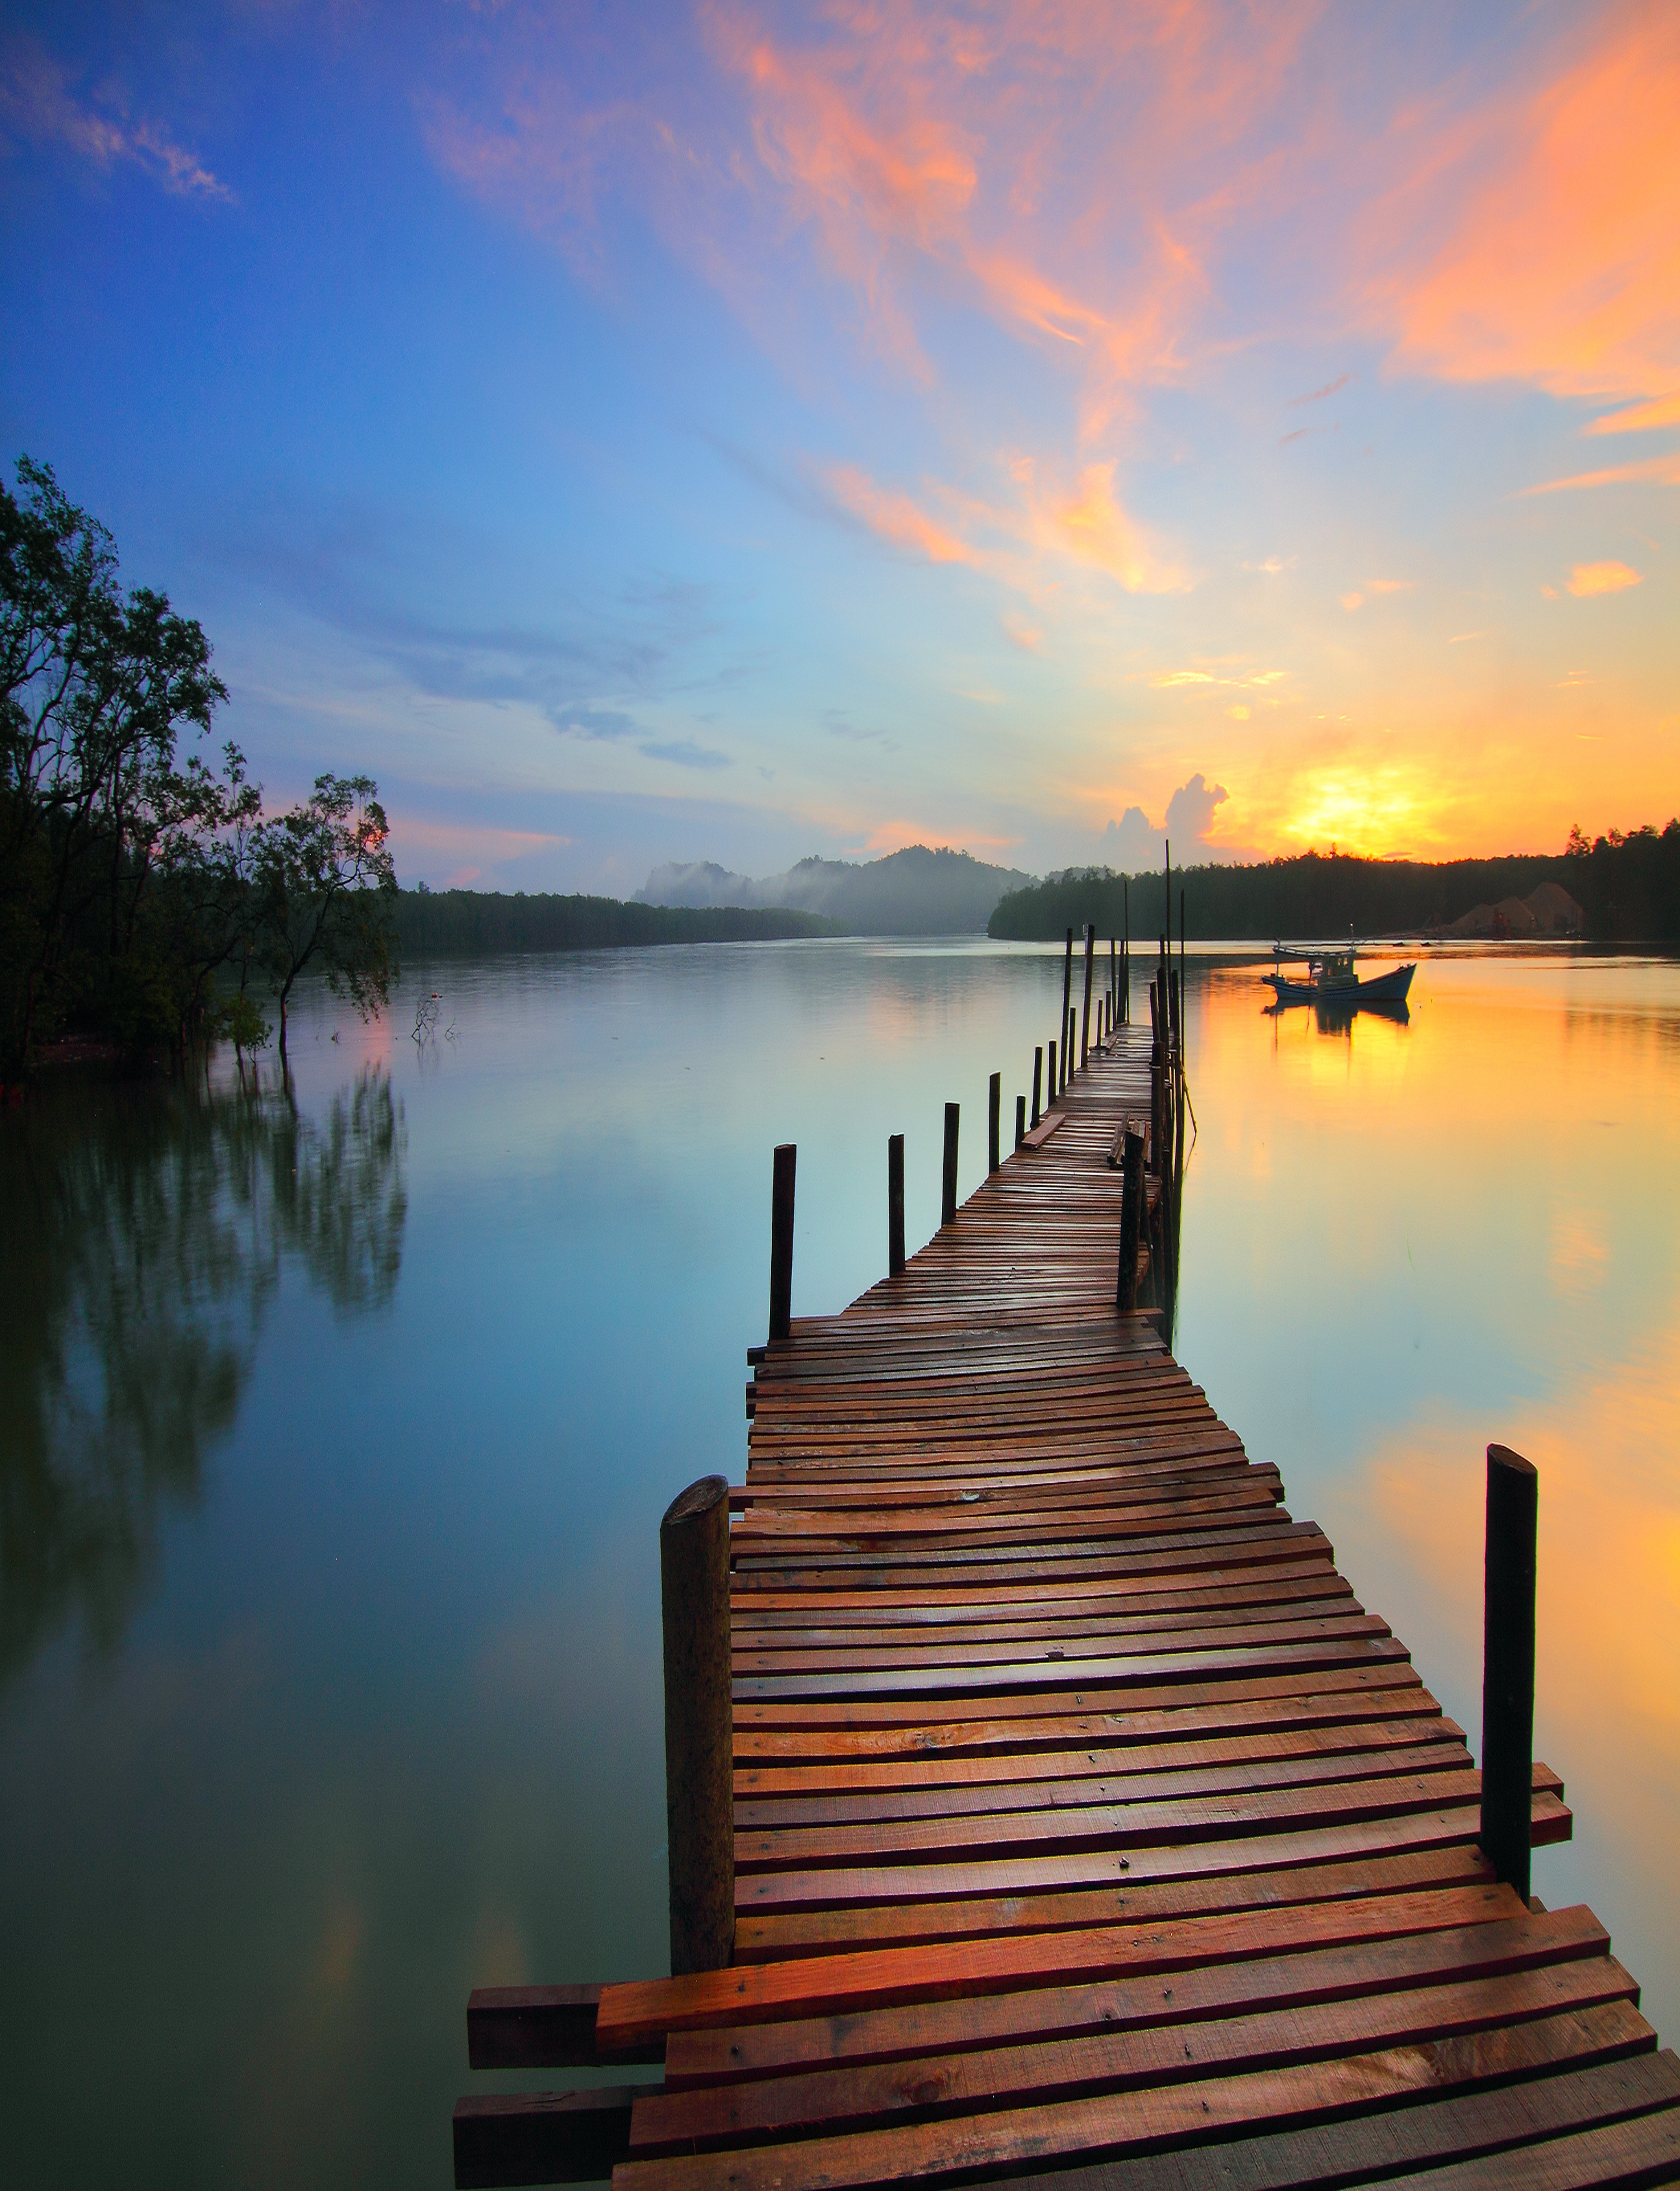
\includegraphics[height=\paperheight,width=8.5in+\bleed]{figures/titlepage-image-print1}%
      }%
    }%
  }
}{
  \backgroundsetup{
    scale=1,
    angle=0,
    opacity=1,
    contents={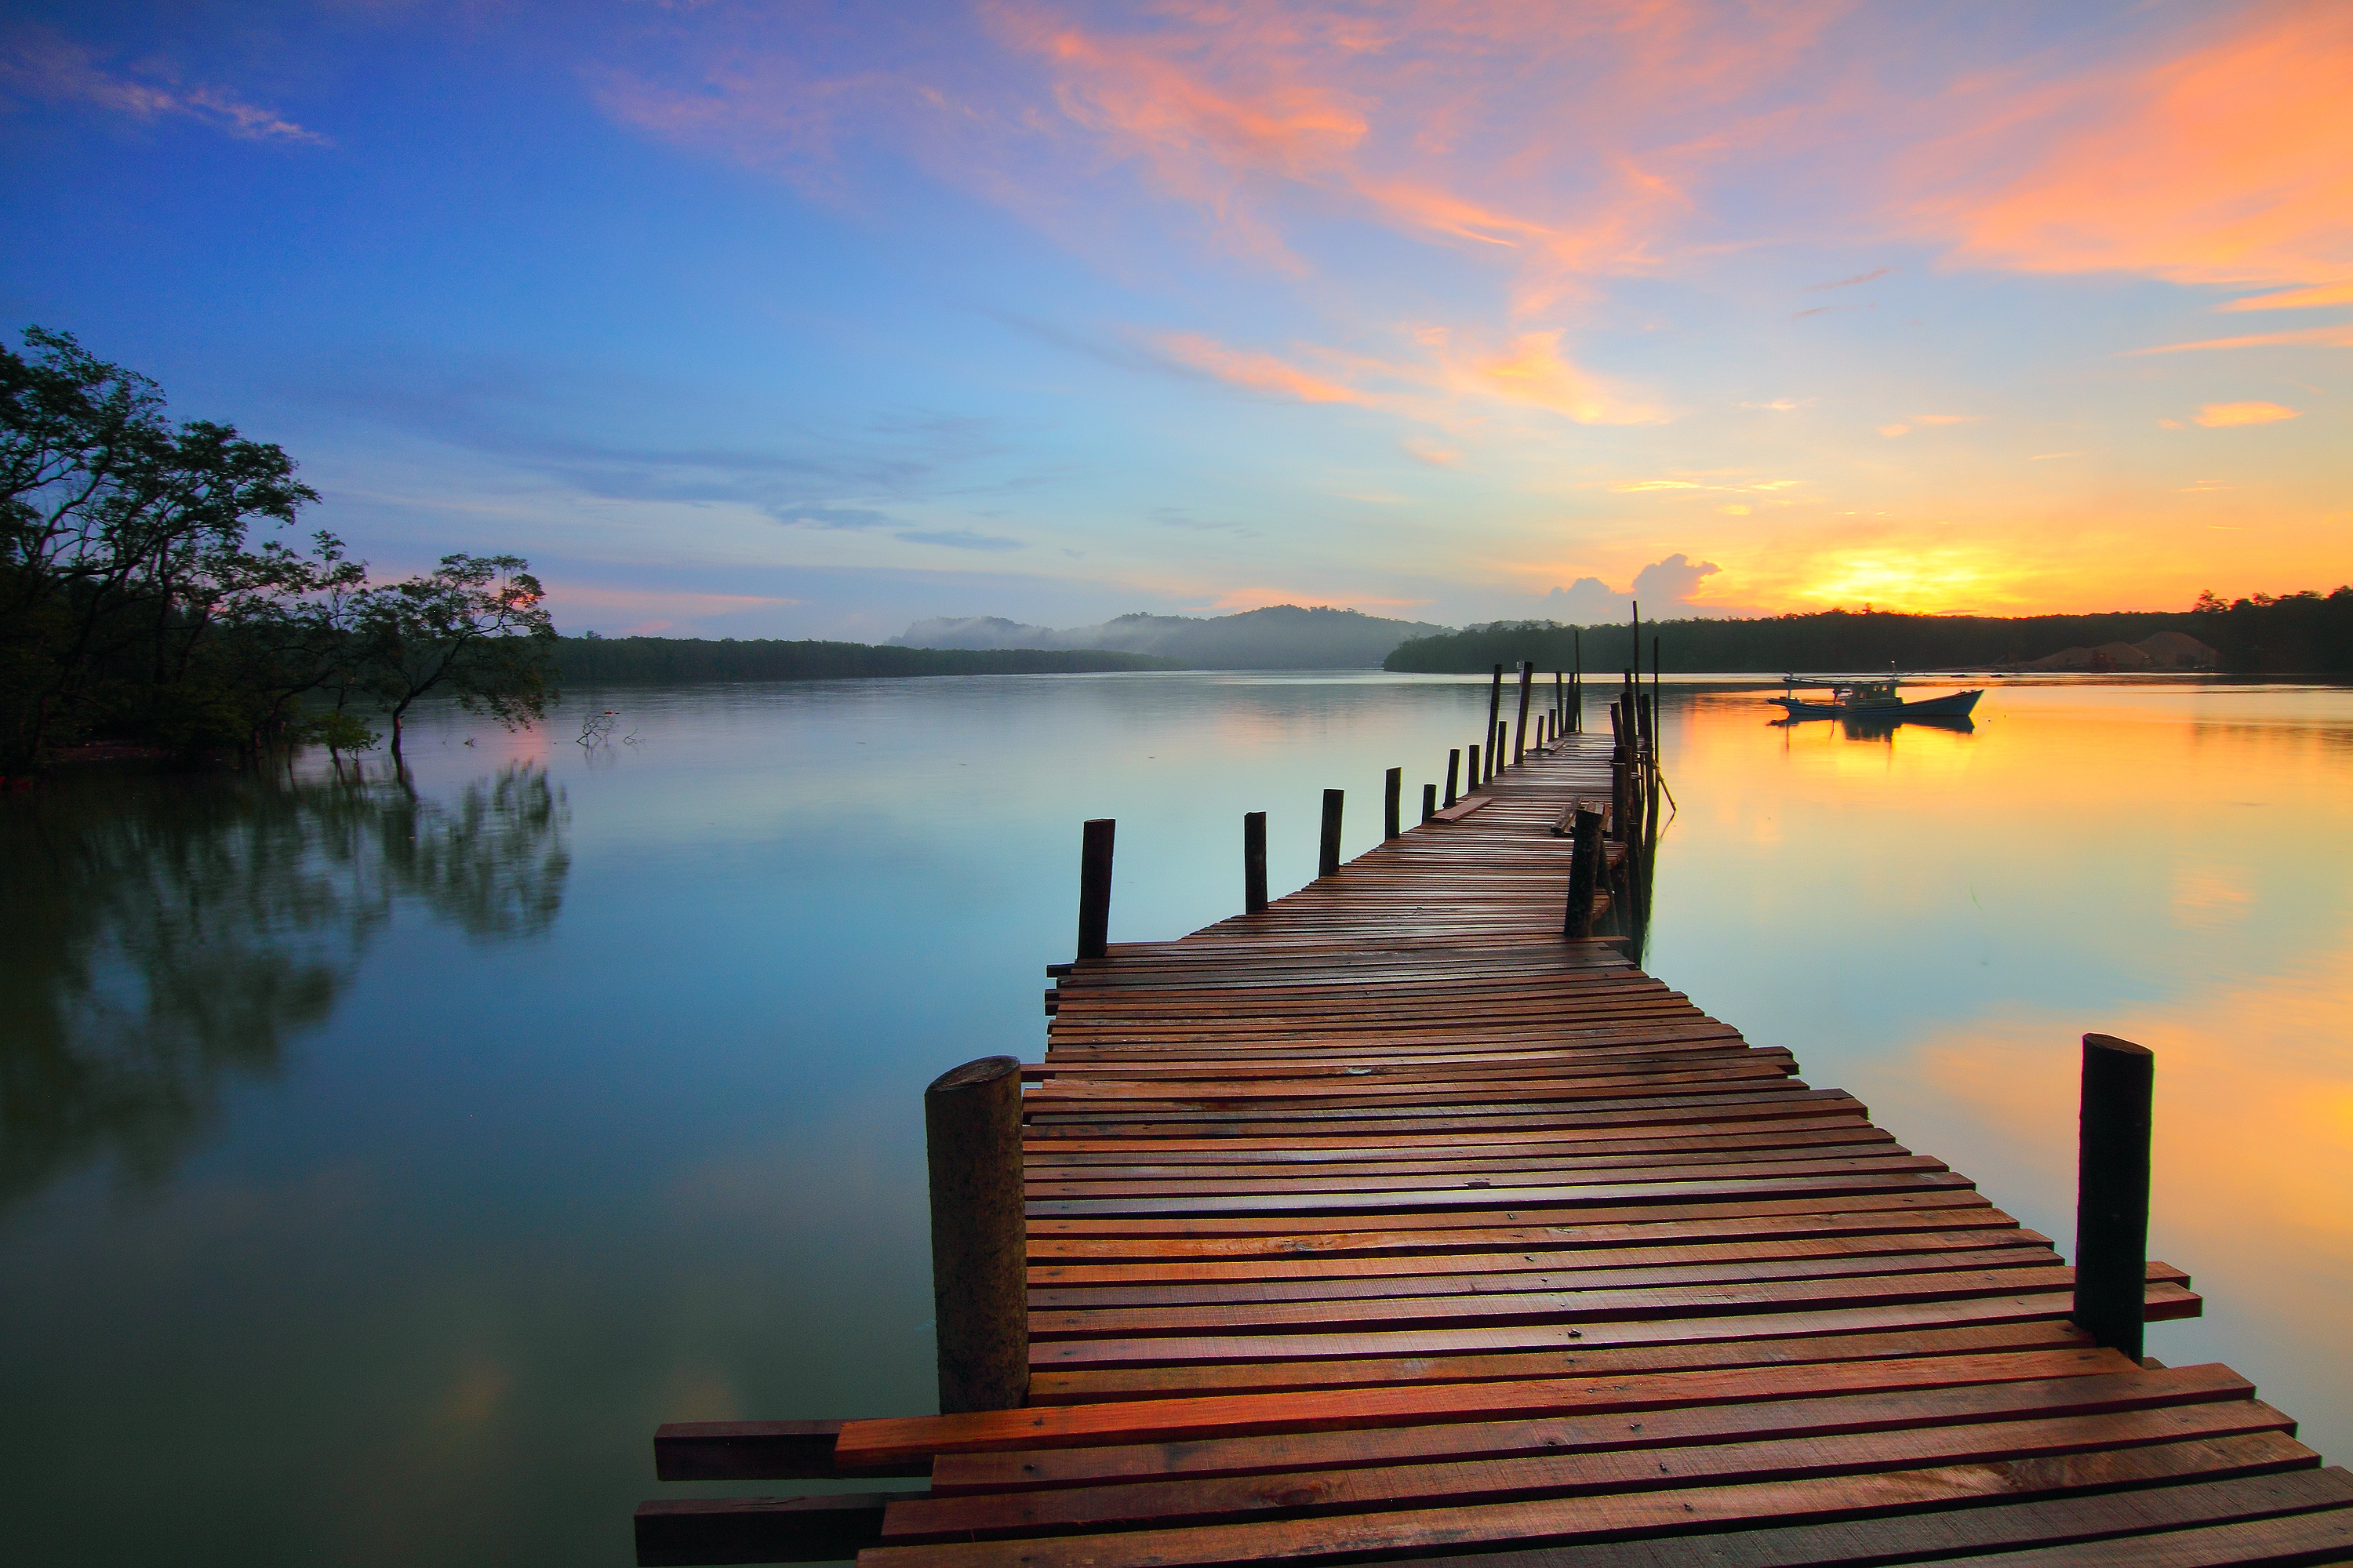
\includegraphics[width=\paperwidth,height=\paperheight]{figures/titlepage-image}}
  }
}  
\BgThispage

%% No page number
\thispagestyle{empty}

%% Title Information
%% Fix spacing on print-cover
\ifthenelse{\equal{\detokenize{print-cover}}{\jobname}}{
  \vspace{1.5em}
}{
  \vspace{7em}
}

\begin{center}
  \textbf{
    \fontsize{34}{36}\selectfont {\textcolor{subtitletextcolour}{\booksubtitle}} \\
    \fontsize{54}{60}\selectfont {\textcolor{titletextcolour}{\booksubject}} \\[.5\baselineskip]
    \fontsize{20pt}{22pt}\selectfont {\textcolor{subtitletextcolour}{An open text by Peter Selinger}}\smallskip\\
    \fontsize{14pt}{18pt}\selectfont {\textcolor{subtitletextcolour}{Based on the original text by Lyryx Learning and Ken Kuttler}}\bigskip \\[.5\baselineskip]
    \fontsize{14pt}{16pt}\selectfont {\textcolor{subtitletextcolour}{\edition}} \\
  }
\end{center}

\vfill

% License
\begin{center*}
  \ifthenelse{\equal{\detokenize{print-cover}}{\jobname}}{
    \raisebox{-0.5in}[0in][0in]{%
      \fontsize{12pt}{12pt}\selectfont \textcolor{cctextcolour}{\textbf{Creative Commons License (CC BY)}}%
    }
  }{
    \fontsize{12pt}{12pt}\selectfont \textcolor{cctextcolour}{\textbf{Creative Commons License (CC BY)}}%
  }
\end{center*}

\ifthenelse{\equal{\detokenize{print-cover}}{\jobname}}{
  \begin{tikzpicture}[remember picture,overlay]
    \node[outer sep=0in, inner sep=0in, anchor=north] at
    ([yshift=-0.25in-\bleed-1in,xshift=\bleed+4.25in]current page.north west) {
      \begin{minipage}{5.2in}
        \setlength{\parskip}{2ex}
        \fontsize{12pt}{16pt}\selectfont
        \textbf{\textsf{
          \textcolor{subtitletextcolour}{
            % The blurb for the back cover

\textit{\bookfulltitle} presents an introduction to the fascinating
subject of linear algebra. It is intended for students in the first or
second year of university, and contains enough material for a
2-semester course. Major topics of linear algebra are presented in
detail, and many applications are given. Although it is not a
proof-oriented book, proofs of most important theorems are
provided. 

\textit{\bookfulltitle} is an open text, and anybody is permitted to
copy and redistribute this book in any medium or format under the
terms of the Creative Commons CC~BY~4.0 License.

          }
        }}
      \end{minipage}
    };
  \end{tikzpicture}
  \begin{tikzpicture}[remember picture,overlay]
    \node[outer sep=0in, inner sep=0in, anchor=center] at
    ([yshift=-0.25in-\bleed-5.5in,xshift=\bleed+8.5in+0.5\spinewidth]current page.north west) {
      \rotatebox{-90}{%
        \begin{minipage}{10in}
          \begin{tikzpicture}
            \node[anchor=west] at (0in,0) {
              \fontsize{26}{28}\selectfont {\textcolor{subtitletextcolour}{\textbf{\textsf{\bookfulltitle}}}}
            };
            \node[anchor=east] at (10in,0) {
              \fontsize{20pt}{22pt}\selectfont {\textcolor{subtitletextcolour}{\textsf{Peter Selinger}}}
            };
          \end{tikzpicture}
        \end{minipage}
      }
    };
  \end{tikzpicture}
}{
  % No back cover for regular pdf
}

